%
% listing2.tex -- the main file of differential and integral advanced calculus notes.
%
% Copyright © 2018 Oromion <caznaranl@uni.pe>
%
% This program is free software: you can redistribute it and/or modify
% it under the terms of the GNU General Public License as published by
% the Free Software Foundation, either version 3 of the License, or
% (at your option) any later version.
%
% This program is distributed in the hope that it will be useful,
% but WITHOUT ANY WARRANTY; without even the implied warranty of
% MERCHANTABILITY or FITNESS FOR A PARTICULAR PURPOSE.  See the
% GNU General Public License for more details.
%
% You should have received a copy of the GNU General Public License
%s along with this program.  If not, see <http://www.gnu.org/licenses/>.
% 
% Please contact caznaranl@uni.pe to report any problems or bugs.
%
\documentclass[12pt,a4paper]{article}
\usepackage[T1]{fontenc}
\usepackage[spanish,es-sloppy]{babel}
\usepackage[pdftex]{graphicx}
\usepackage[dvipsnames, usenames]{color}
\usepackage[lmargin=2.5cm,rmargin=2.5cm,tmargin=2cm,bmargin=3cm]{geometry}
\usepackage[shortlabels]{enumitem}
\usepackage{url,here}

\linespread{1.5}
\setlength{\parindent}{5mm}

\title{\scshape Juegos de mesa}
\author{Juan Pérez\thanks{Gracias a CTIC}}
\date{agosto, 22 del 2016}
\graphicspath{{../images/}}

\begin{document}

\maketitle
\tableofcontents
\listoffigures
\listoftables

\begin{abstract}
Esta es la primera práctica para LaTeX 2016-III, que debe ser entregado a más tardar el miércoles 24 de agosto a las 15:00 hrs. Las imágenes se encuentran en

\url{http://www.bbc.com/mundo/noticias/2011/01/110126_cerebro_juegos_mesa_men}
\end{abstract}

\section{Los expertos en juegos de mesa usan mejor el cerebro (Ver Figura \ref{fig:1})}

\begin{figure}[H]
	\centering
	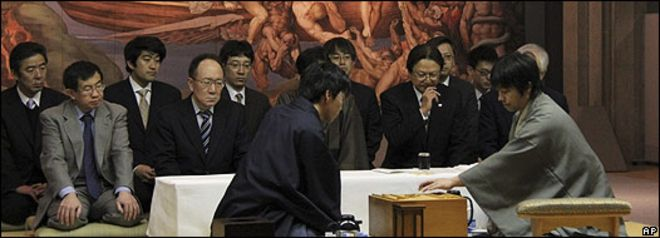
\includegraphics[scale=0.5]{fig1}
	\caption{Los científicos estudiaron a expertos en shogi, el ajedrez japonés.}\label{fig:1}
\end{figure}

{\bfseries Una nueva investigación descubrió que los expertos en juegos de mesa, como el ajedrez\footnote{Ver figura \ref{fig:2}}, utilizan una región del cerebro que el resto no solemos usar.}

{\sffamily El estudio, publicado en Science, llevó a cabo escáneres cerebrales de jugadores, tanto profesionales como aficionados, del juego japonés shogi, también llamado ajedrez japonés debido a su similitud.}

Los investigadores del Instituto de Ciencia Cerebral Riken, en Japón, descubrieron que las jugadas intuitivas que llevan a cabo estos jugadores no son naturales, sino que surgen del entrenamiento cerebral.

Los profesionales del shogi entrenan hasta por 10 años, tres o cuatro horas al día, para lograr la habilidad que se requiere para jugar a ese nivel.

\begin{flushright}
El hallazgo fue una sorpresa, porque al volverse expertos los maestros shogi comienzan a usar todas las regiones del cerebro
Prof. Keiji Tanaka
\end{flushright}

Estos individuos son capaces de llevar a cabo decisiones "intuitivas" muy rápidas sobre la jugada o combinación de jugadas que harán en el tablero para lograr el mejor resultado.

\begin{figure}[H]
	\centering
	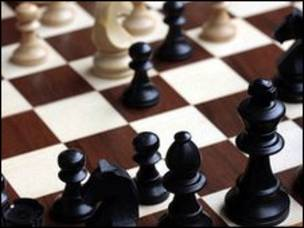
\includegraphics[scale=0.5]{fig2}
	\caption{Quienes juegan profesionalmente utilizan partes del cerebro que otros no usan.}\label{fig:2}
\end{figure}

Los científicos reclutaron a jugadores profesionales miembros de la Asociación Japonesa de Shogi.

También participó en el estudio un grupo de jugadores aficionados.

A 17 de los profesionales se les presentó un juego de shogi que ya estaba en progreso y se les dieron dos segundos para elegir la mejor jugada siguiente, de entre cuatro jugadas.

{\Large Según los investigadores, los escáneres cerebrales de estos jugadores mostraron una activación significativa en el área del núcleo caudado mientras llevaban a cabo sus jugadas rápidas.}

Durante mucho tiempo se ha pensado que esa región del cerebro es responsable del control de los movimientos corporales voluntarios. Pero estudios más recientes lo han vinculado al aprendizaje y la memoria.

\subsection{Actividad cerebral}

Cuando se les pidió a los jugadores aficionados que eligieran rápidamente su mejor jugada siguiente, no se observó activación significativa en el núcleo caudado.

Esta actividad cerebral sólo se vio en los jugadores profesionales que llevaban a cabo decisiones muy rápidas sobre la siguiente mejor jugada.

Además, se encontró que los profesionales no usaban esa área del cerebro cuando se les daba un tiempo mayor a los ocho segundos para que pensaran estratégicamente sobre las siguientes jugadas que debían realizar.

Con este escenario no se activaba el área del núcleo caudado cerebral.

{\color{red} El profesor Keiji Tanaka, quien dirigió el estudio, dijo haberse sorprendido por el hallazgo ya que esta zona del cerebro, que forma parte de los ganglios basales, no está asociada con la inteligencia.}

"Los jugadores profesionales comenzaron a usar partes del cerebro que están bien desarrolladas en ratones y ratas pero no tan desarrolladas en los primates", dice el científico.

``Así que el hallazgo fue una sorpresa, porque al volverse expertos los maestros shogi comienzan a usar todas las regiones del cerebro''.

{\flushright\underline{Según el profesor Tanaka}, el hallazgo confirma la idea de que el cerebro puede ser entrenado para detectar patrones, y es poco probable que la gente nazca con la capacidad de intuición necesaria para ser un experto en juegos de mesa.}

\section{Una tabla}

La siguiente tabla (Ver \cite{Vo11}) tiene las siguientes entradas.

\begin{enumerate}
	\item ab
	\item cd
	\begin{enumerate}[$\bullet$]
		\item uno
		\item dos
		\item tres
	\end{enumerate}
	\item ef
	\item ghi
	\item j
	\item k
	\item lm
\end{enumerate}


\begin{table}[H]
\centering
\caption{La siguiente tabla es muy simple}
\begin{tabular}{|r|c|l|}
\hline
\multicolumn{3}{|c|}{Una tabla simple} \\
\hline
ab & cd & ef \\
\cline{1-2}
\multicolumn{2}{|c|}{ghi} &  \\
\hline
j & k & lm \\
\hline
\end{tabular}
\end{table}

\begin{thebibliography}{99}
	\bibitem{Vo11} Vo\ss, Herbert. \emph{Typesetting tables with \LaTeX}. UIT Cambridge, 2011.
\end{thebibliography}

\end{document}